% ------------------------------------------------------------------------------
% includes preamble stuff
\documentclass[a4paper,11pt]{report}
%\documentclass[a4paper,11pt]{article}

% sans serif font 
%\renewcommand{\familydefault}{\sfdefault}


%title page stuff
\newcommand{\HRule}{\rule{\linewidth}{0.5mm}}

% margins
\usepackage[top=2.5cm, bottom=2.5cm, left=4cm, right=2.5cm]{geometry}
\geometry{a4paper} % or letterpaper (US) or a5paper or....
%\geometry{margin=1in}

\usepackage{fancyhdr}
\pagestyle{fancyplain}
\fancyfoot[C]{\thepage}                 % page number in centre of foot.
\fancyfoot[R]{\small{M. J. Hawes, 10238908}}	% right of footer. 
\rhead{}

% \usepackage{setspace}           
% \onehalfspacing               % Sets the line spacing to 1.5


% ------------------------------------------------------------------------------
% provides comment functionality
\usepackage{verbatim}

% ------------------------------------------------------------------------------
% setting up harvard style refs
%\usepackage{harvard}
%\bibliographystyle{harvard}
\bibliographystyle{plain}

\usepackage{cite}

% ------------------------------------------------------------------------------
% needed for code listings
\usepackage{color}
\usepackage{xcolor}
\usepackage{listings}

\usepackage{caption}
\DeclareCaptionFont{black}{\color{black}}
\DeclareCaptionFormat{listing}{\colorbox{white}{\parbox{\textwidth}{#1#2#3}}}
\captionsetup[lstlisting]{format=listing,labelfont=black,textfont=black}

\lstset{ %
language=C,                % choose the language of the code
basicstyle=\footnotesize,       % the size of the fonts that are used for the code
numbers=left,                   % where to put the line-numbers
numberstyle=\footnotesize,      % the size of the fonts that are used for the line-numbers
stepnumber=1,                   % the step between two line-numbers. If it is 1 each line will be numbered
numbersep=5pt,                  % how far the line-numbers are from the code
backgroundcolor=\color{black!6!white},  % choose the background color. You must add \usepackage{color}
showspaces=false,               % show spaces adding particular underscores
showstringspaces=false,         % underline spaces within strings
showtabs=false,                 % show tabs within strings adding particular underscores
frame=single,           % adds a frame around the code
tabsize=2,          % sets default tabsize to 2 spaces
captionpos=b,           % sets the caption-position to bottom
breaklines=true,        % sets automatic line breaking
breakatwhitespace=true,    % sets if automatic breaks should only happen at whitespace
%escapeinside={\%*}{*)}          % if you want to add a comment within your code
}

% ------------------------------------------------------------------------------
% Graphics stuff for images
\usepackage{graphicx}
\DeclareGraphicsExtensions{.jpg,.jpeg,.png}
\graphicspath{ {./imgs/} }

% for graphs
\usepackage{tikz}
\usepackage{pgfplots}

\usepackage{epstopdf}		% .eps to .pdf

\usepackage{float}
%\floatstyle{boxed}
\restylefloat{figure}
\usepackage{caption}
\usepackage{subcaption}

\renewcommand{\thesubfigure}{\roman{subfigure}}
\captionsetup[subfigure]{labelformat=simple, labelsep=colon}

% Caption stuff
\begin{comment}
\DeclareCaptionFormat{myformat}{%
  \colorbox{lightgray!30}{\parbox{\dimexpr\textwidth-2\fboxsep-2\fboxrule\relax}{#1#2#3}}
} 
\captionsetup[figure]{format=myformat}
\captionsetup[lstlisting]{format=myformat}
\captionsetup[table]{format=myformat}
\end{comment}

% ------------------------------------------------------------------------------
% Maths packages
\usepackage{amsmath}

% ------------------------------------------------------------------------------
% Glossary packages
\newcommand*{\glossfirstformat}[1]{\textbf{#1}}

\usepackage[]{glossaries}
\renewcommand*{\glspostdescription}{}
\glossarystyle{list}
\makeglossaries

\renewcommand{\glsdisplayfirst}[4]{\glossfirstformat{#1#4}}
\renewcommand*{\glsnamefont}{\sffamily}
\renewcommand*{\glossarymark}[1]{}

\newglossaryentry{Makefile}
{
    name={Makefile},
    description={},
    plural={Makefiles}
}

\newglossaryentry{thread}
{
    name={thread},
    description={},
    plural={threads}
}

\newglossaryentry{multi-threaded algorithm}
{
    name={multi-threaded algorithm},
    description={},
    plural={multi-threaded algorithms}
}

\newglossaryentry{scheduling}
{
    name={scheduling},
    description={},    
}

\newglossaryentry{worker-thread}
{
    name={worker-thread},
    description={},
    plural={worker-threads}
}

\newglossaryentry{monitor-thread}
{
    name={monitor-thread},
    description={},
    plural={monitor-threads}
}

\newglossaryentry{mutex}
{
    name={mutex},
    description={},
    plural={mutexes}
}

\newglossaryentry{barrier}
{
    name={barrier},
    description={},
    plural={barriers}
}

\newglossaryentry{conditional-variable}
{
    name={conditional-variable},
    description={},
    plural={conditional-variables}
}
\newglossaryentry{load-balancing}
{
    name={load-balancing},
    description={},
}

\newglossaryentry{work-stealing}
{
    name={work-stealing},
    description={A processor which is starved of work attempts to ``steal'' 
                 work from other processors},
}

\newglossaryentry{thief}
{
    name={thief},
    description={},
    plural={thieves}
}

\newglossaryentry{victim}
{
    name={victim},
    description={},
    plural={victims}
}

\newglossaryentry{ready-deque}
{
    name={ready-deque},
    description={},
    plural={ready-deques}
}

\newglossaryentry{non-blocking}
{
    name={non-blocking},
    description={},
}

\newglossaryentry{steal-operation}
{
    name={steal-operation},
    description={},
}

\newglossaryentry{work-sharing}
{
    name={work-stealing},
    description={A processor which creates new work attempts to migrate it to 
                 another underutilised processor at creation time},
}

\newglossaryentry{locality}
{
    name={locality},
    description={},
}

\newglossaryentry{julia-set}
{
    name={julia-set},
    description={},
    plural={julia-sets}
}

\newglossaryentry{filled julia-set}
{
    name={filled julia-set},
    description={},
    plural={filled julia-sets}
}

\newglossaryentry{critical-orbit}
{
    name={critical-orbit},
    description={},
    plural={critical-orbits}
}

\newglossaryentry{fractal}
{
    name={fractal},
    description={},
    plural={fractals}
}

\newglossaryentry{complex-number}
{
    name={complex-numer},
    description={},
    plural={complex-numbers}
}

\newglossaryentry{real-world-fractal}
{
    name={real-world-fractal},
    description={},
    plural={real-world-fractals}
}

\newglossaryentry{mathematical-fractal}
{
    name={mathematical-fractal},
    description={},
    plural={mathematical-fractals}
}

\newglossaryentry{scale-invariance}
{
    name={scale-invariance},
    description={},
}

\newglossaryentry{self-similarity}
{
    name={self-similarity},
    description={},
}

\newglossaryentry{exact self-similarity}
{
    name={exact self-similarity},
    description={},
}

\newglossaryentry{quasi self-similarity}
{
    name={quasi self-similarity},
    description={},
    plural={quasi self-similar}
}



% ------------------------------------------------------------------------------
% Appendix packages
\usepackage[toc,page]{appendix}

\makeatletter
    \def\thebibliography#1{\chapter*{References\@mkboth
      {REFERENCES}{REFERENCES}}\list
      {[\arabic{enumi}]}{\settowidth\labelwidth{[#1]}\leftmargin\labelwidth
	\advance\leftmargin\labelsep
	\usecounter{enumi}}
	\def\newblock{\hskip .11em plus .33em minus .07em}
	\sloppy\clubpenalty4000\widowpenalty4000
	\sfcode`\.=1000\relax}
    \makeatother


% ------------------------------------------------------------------------------
%title
\title{
\huge Work-Stealing Scheduling Techniques Applied to Computing the Mandelbrot Set.
}

\author{
  Martin J Hawes\\
  \\
  Department of Computer Science, \\
  The University of Hertfordshire \\ 
  \\
  \textit{hawesmartin@googlemail.com}\\
}

% ------------------------------------------------------------------------------
% - Document starts here
% ------------------------------------------------------------------------------

\begin{document}
\maketitle
\date{}
\pagenumbering{Roman}

% ---------------------------------------------------------------------------------------------------------------------------------------------------------------
\section*{Abstract}


% ---------------------------------------------------------------------------------------------------------------------------------------------------------------
\section*{Acknowledgements}

% ---------------------------------------------------------------------------------------------------------------------------------------------------------------
\clearpage
\pagenumbering{arabic}
\setcounter{page}{1}
\tableofcontents

% ---------------------------------------------------------------------------------------------------------------------------------------------------------------
% ---------------------------------------------------------------------------------------------------------------------------------------------------------------
% ---------------------------------------------------------------------------------------------------------------------------------------------------------------
\chapter{Introduction}

% Identify subject area and clearly state the arena of interest this report investigates.
    % * state of the field. 
    % * Talk about highly parallel computing and its applications. Be broad.

Multi-processor computers are now commonplace in the world of computing, for both consumers and scientists alike. 
This shift in architectural design demands a drastic shift in how a program is constructed, from the standpoint of both
the programmer and the language designer.

\section*{Motivation}



\section*{Aim}

To investigate, through research and practical implementation, the effectiveness of work-stealing run-time scheduling on
a parallel algorithm which computes an approximation of the Mandelbrot set.

\section*{Objectives}
This section outlines the deliverable items that are presented in this report.
Core objectives are primary and more vital, advanced objectives are additional items.

\subsection*{Core Objectives}
\newcounter{saveenum}
\begin{enumerate}
\item \textbf{Background Research}
\item \textbf{A Sequential Mandelbrot Set Algorithm}
\item \textbf{A Random Work-Stealing Mandelbrot Set Algorithm}
\item \textbf{A Render Thread Work-Stealing Mandelbrot Set Algorithm}
\item \textbf{Cross Analysis of the Implemented Algorithms}
\setcounter{saveenum}{\value{enumi}}
\end{enumerate}

\subsection*{Advanced Objectives}
\begin{enumerate}
\setcounter{enumi}{\value{saveenum}}
\item \textbf{Work-Stealing Trace System:}
\end{enumerate}

\section*{Achievements}
The following table shows each objective and its final completion status at the time this 
report was finalised. 

\begin{table}[H]
    \centering
    \begin{tabular}{|r|l|}
        \hline
            \textbf{Objective} & \textbf{Status} \\
        \hline \hline
            \textbf{1} & Complete \\
            \textbf{2} & Complete \\
            \textbf{3} & Complete \\
            \textbf{4} & Partially Complete \\
            \textbf{5} & - \\
        \hline
            6 & - \\
        \hline
    \end{tabular}
    
    \label{tab:ach}
    \caption{Table of Achievements}
\end{table}

\section*{Report Structure}

There are five remaining chapters in this report. 
In chapter two a detailed review of the problem background is presented. 
Chapter three details the practical implementation, which this report is based on, including validation and verification of the described software.
Chapter four offers an evaluation of the project as a whole. This includes analysis of the implemented software and a comparison of the implemented
schemes.
Chapter five lists the resources referenced in this report.
In chapter six the appendices are presented.

A glossary of terms is presented as Appendix A. 
This consists of a list describing major concepts surrounding the field of study, and directs the reader to their pages of occurrence. 

The source code for all software developed to fulfil the objectives described above is presented as Appendix B.



% Identify some of the key pieces of literature or applications for the subject area I have chosen.
% This report identifies two contrasting work-stealing schemes and analyses their performance using an algorithm to
% compute an approximation of the Mandelbrot set as a case study. 

% Talk about the specific investigated area's and what the report specifically talks about.
    % * i.e. which work-stealing schemes are implemented, which Mandelbrot algorithm is identified.

% Rationale for doing above said things and aims of project.
% The work is carried out in order to establish an understanding of how effective run-time scheduling of parallel 
% computations is when considering load-balancing. 

% Disclaimer section i.e. This report assumes prior knowledge of blah blah blah and is written
%   with whomever in mind and so on.
% This report assumes some prior understanding of parallel algorithms.

% ---------------------------------------------------------------------------------------------------------------------------------------------------------------
% ---------------------------------------------------------------------------------------------------------------------------------------------------------------
% ---------------------------------------------------------------------------------------------------------------------------------------------------------------
\chapter{Background Research}
% ---------------------------------------------------------------------------------------------------------------------------------------------------------------

\section{Run-Time Scheduling Techniques for Multi-Threaded Computations}
This section briefly describes the problems associated with \gls{scheduling} \glspl{multi-threaded algorithm} at run-time and
the major paradigms that have surfaced.

% explain problems here...... is this better off in the intro??
To efficiently utilise a parallel computer architecture it is desirable to minimise
the amount of time a processor spends idle or performing other logistical tasks, i.e not doing work. 
When a computation's concurrent sub-tasks or \glspl{thread} incur a regular cost in processor
time, each processor can simply have the same amount of work assigned to them. When the computation has
more irregular or dynamically growing sub-tasks a problem arises resulting in 
processors becoming idle while others still remain working. The solution to this problem is referred to as
\gls{load-balancing} and can be described as a form of dynamic scheduling that ensures each processor 
spends approximately the same amount of time working. This means processors generally spend
less time idle, however have to deal with scheduling overheads as a trade-off.

When considering the scheduling of multi-threaded computations, two major load balancing techniques have been used.
These are \gls{work-sharing} and \gls{work-stealing}.

\begin{itemize}
\item \textbf{Work-Sharing:} A processor which creates new work attempts to migrate it to another underutilised processor at creation time. 
\item \textbf{Work-Stealing:} A processor which is starved of work attempts to ``steal'' work from other processors. 
\end{itemize}

Both techniques intend to promote balanced work-load across all processors, however in Work-Stealing
the frequency of work migrations is lower. When all processors have a 
high work-load and no need to ``steal" this becomes useful because threads need not get 
migrated at all. With \gls{work-sharing} work migration occurs each time new work is created \cite{blumleis}.
This also suggests that \gls{work-stealing} promotes better \gls{locality} and grouping of sub-tasks, as spawned work 
stays with the same processor until stolen.

% ---------------------------------------------------------------------------------------------------------------------------------------------------------------
\section{The Mandelbrot Set}

The Mandelbrot set is a set of complex numbers which when plotted produce a spectacular and recognisable shape as illustrated in figure~\ref{fig:mandelimg}.
It is often presented as a colourful and striking image and has been described by some as the most beautiful object in all of mathematics \cite[p.~234]{chaosfract}.
The \glspl{complex-number} that comprise the set are closely related to \glspl{julia-set}. 
In-fact the Mandelbrot set can be described as a catalogue of Julia Sets which, when plotted, all points are connected, 
forming a single, unbroken shape \cite[p.~177]{fractimg}.

The set is named for the mathematician Benoit Mandelbrot, who discovered it in 1980 \cite{fracnature , fractimg}. He was a pioneer in the study of 
fractal geometry and also coined the term \gls{fractal}, of which both the Mandelbrot set, and Julia sets are examples of. 

In this section I will give a more detailed explanation of the areas mentioned here. 

\begin{figure}[h]
  \caption{A rendering of The Mandelbrot Set generated using the program ``fraqtive"\cite{fraqtive}.}
  \label{fig:mandelimg}
  \centering
    
\includegraphics[width=1\textwidth]{mandelbrot}
\end{figure}

\subsection*{Fractals and Self-Similarity} 
%TODO: this section needs citations all over the shop!
A \gls{fractal} is a means of describing shapes which are more complex than classical geometric shapes. The leaves of a pine tree or the forks of a 
lightning bolt are obvious examples of real things that fractals allow us to more faithfully describe. 
These \glspl{real-world-fractal} are similar to \glspl{mathematical-fractal}, 
of which the Mandelbrot set is an example, but differ in that they do not display the property of \gls{scale-invariance}. 

Fractals have a fractional dimension. Unlike shapes with topological dimension, for instance a two dimensional square, 
a \glspl{fractal} dimension is of a non integer value.

A property of fractals (but not all) is \gls{self-similarity}, where the shape is comprised of smaller ``copies" of itself. 
This is known as \gls{exact self-similarity} and means the shape is identical at any scale.
A well-known example of this is the Triadic Koch Snowflake which is a fractal constructed using equilateral triangles. 
It is important to note here that The Mandelbrot set does not quite show the same property, it is said to be 
\glspl{quasi self-similarity}. This means the shape is approximately similar at all scales, in that the shape is replicated but in a slightly distorted
form with each ``copy".

%TODO
It turns out there are many rather useful applications for fractals. To name a few; computer game graphics, %FIND MORE EXAMPLES WITH CITATIONS.

\subsection*{Julia Sets}

To understand the basis of the Mandelbrot set it is first necessary to understand it's relation to \glspl{julia-set}.
The function in equation~\ref{eq:julia1} is iterated infinitely where \(c\) is fixed.
The \gls{filled julia-set} is comprised of all values of \(z_0\) where the result is bounded and does not tend towards infinity.
The \gls{julia-set} is comprised of those members of the \gls{filled julia-set} which lie on the boundary \cite{chaosfract}.
In the interest of keeping this report readable, and because filled Julia Sets are more relevant, \glspl{filled julia-set} will be 
referred to simply as \glspl{julia-set}.

% express the set notation for f(x) -> infinity.???? TODO
\begin{equation}\label{eq:julia1}
f(z) = z^2 + c
\end{equation}

With regards to the Mandelbrot Set I am interested in \glspl{julia-set} in which the values \(c\) and \(z\) used are expressed as a 
\gls{complex-number}. Figure~\ref{fig:juliaimgs} illustrates some examples of such sets. 

\begin{figure}[h]
\centering
\begin{subfigure}[b]{0.48\textwidth}
  \centering    
  
\includegraphics[width=\textwidth]{julia-con}
  \caption{
    \tiny The \gls{julia-set} where \(c = -0.1 + 0.649i\)
  }
  \label{fig:juliaimgcon}
\end{subfigure}
~ %spacer
\begin{subfigure}[b]{0.48\textwidth}
  \centering
  
\includegraphics[width=\textwidth]{julia-ncon}
  \caption{
    \tiny The \gls{julia-set} where \(c = -0.75 + 0.03i\)
  }
  \label{fig:juliaimgncon}
\end{subfigure}
% full caption
\caption{
  Two Julia Sets rendered using the program ``fraqtive"\cite{fraqtive}. 
  Figure~\ref{fig:juliaimgcon} is a member of the Mandelbrot set, 
  figure~\ref{fig:juliaimgncon} is not.
}
\label{fig:juliaimgs}
\end{figure}

\subsection*{Computing the Mandelbrot Set}

The set is comprised of those \glspl{julia-set} which are connected. In order to determine whether a Julia Set possesses this property,
we need only compute the result for \(z_0\). If this tends towards infinity the value \(c\) is not a member of the Mandelbrot Set. If the result
is bounded, then it is a member. This is known as the \gls{critical-orbit} and is useful because it means we do not have to compute
the entire Julia Set for each value of \(c\).

So the Mandelbrot set can be computed by iterating all possible values of \(c\) for the function in equation~\ref{eq:julia1} where \(z\) is the 
\gls{critical-orbit}. Because the set of all possible values of \(c\) is infinite, and computers have a finite amount of resources, this 
set needs to be approximated. This can be done using a raster plane which takes samples of the complex plane at regular intervals. 

% TALK ABOUT VARIOUS ALGORITHMS PRESENTED TODO
Level set method \cite[p.~188]{fractimg} Continuous Potential Method \cite[p.~191]{fractimg}

% ---------------------------------------------------------------------------------------------------------------------------------------------------------------
\section{The Work-Stealing Technique - Described in Depth}

As described above, \gls{work-stealing} is a \gls{load-balancing} technique which allows work starved processors to acquire scheduled work from other processors. 

Each processor has a number of assigned tasks to complete. In general, a processor acquires its work from here.
However, once these tasks are exhausted, the processor becomes a \gls{thief} and chooses a \gls{victim} to steal from. 
The method used to choose a victim is implementation specific, for instance some implementations adopt a random scheme \cite{blumleis , jliff, narora}.
If the processor successfully steals work it relinquishes its thief state and returns to doing work.
If the steal attempt is unsuccessful, for instance when the victim has no work or is blocked, the processor tries again
until it is determined that there is no work remaining in the entire network. 

Figure~\ref{fig:stealoperation} illustrates the result of a successful steal operation in which work-starved processor \textit{p1} transfers a piece
of work from \textit{p0's} work list to its own. %do more here.

\begin{figure}[h]
\centering
\begin{subfigure}[b]{0.4\textwidth}
  \centering    
%  \includegraphics[width=\textwidth]{stealreq}
  % Graphic for TeX using PGF
% Title: /media/martin/69f663af-aa17-4b22-836c-5646358695f1/fyp/wstealmandel/writeup/diagrams/stealreq.dia
% Creator: Dia v0.97.2
% CreationDate: Fri Feb 15 17:19:52 2013
% For: martin
% \usepackage{tikz}
% The following commands are not supported in PSTricks at present
% We define them conditionally, so when they are implemented,
% this pgf file will use them.
\ifx\du\undefined
  \newlength{\du}
\fi
\setlength{\du}{15\unitlength}
\begin{tikzpicture}
\pgftransformxscale{1.000000}
\pgftransformyscale{-1.000000}
\definecolor{dialinecolor}{rgb}{0.000000, 0.000000, 0.000000}
\pgfsetstrokecolor{dialinecolor}
\definecolor{dialinecolor}{rgb}{1.000000, 1.000000, 1.000000}
\pgfsetfillcolor{dialinecolor}
\pgfsetlinewidth{0.100000\du}
\pgfsetdash{}{0pt}
\pgfsetdash{}{0pt}
\pgfsetmiterjoin
\definecolor{dialinecolor}{rgb}{1.000000, 1.000000, 1.000000}
\pgfsetfillcolor{dialinecolor}
\fill (1.000000\du,11.800000\du)--(1.000000\du,13.800000\du)--(3.000000\du,13.800000\du)--(3.000000\du,11.800000\du)--cycle;
\definecolor{dialinecolor}{rgb}{0.000000, 0.000000, 0.000000}
\pgfsetstrokecolor{dialinecolor}
\draw (1.000000\du,11.800000\du)--(1.000000\du,13.800000\du)--(3.000000\du,13.800000\du)--(3.000000\du,11.800000\du)--cycle;
% setfont left to latex
\definecolor{dialinecolor}{rgb}{0.000000, 0.000000, 0.000000}
\pgfsetstrokecolor{dialinecolor}
\node[anchor=west] at (1.600000\du,13.000000\du){p0};
\pgfsetlinewidth{0.100000\du}
\pgfsetdash{}{0pt}
\pgfsetdash{}{0pt}
\pgfsetmiterjoin
\definecolor{dialinecolor}{rgb}{1.000000, 1.000000, 1.000000}
\pgfsetfillcolor{dialinecolor}
\fill (1.000000\du,7.000000\du)--(1.000000\du,10.800000\du)--(3.000000\du,10.800000\du)--(3.000000\du,7.000000\du)--cycle;
\definecolor{dialinecolor}{rgb}{0.000000, 0.000000, 0.000000}
\pgfsetstrokecolor{dialinecolor}
\draw (1.000000\du,7.000000\du)--(1.000000\du,10.800000\du)--(3.000000\du,10.800000\du)--(3.000000\du,7.000000\du)--cycle;
% setfont left to latex
\definecolor{dialinecolor}{rgb}{0.000000, 0.000000, 0.000000}
\pgfsetstrokecolor{dialinecolor}
\node[anchor=west] at (0.000000\du,10.400000\du){};
\pgfsetlinewidth{0.100000\du}
\pgfsetdash{}{0pt}
\pgfsetdash{}{0pt}
\pgfsetbuttcap
{
\definecolor{dialinecolor}{rgb}{0.000000, 0.000000, 0.000000}
\pgfsetfillcolor{dialinecolor}
% was here!!!
\definecolor{dialinecolor}{rgb}{0.000000, 0.000000, 0.000000}
\pgfsetstrokecolor{dialinecolor}
\draw (1.400000\du,8.400000\du)--(2.600000\du,8.400000\du);
}
\pgfsetlinewidth{0.100000\du}
\pgfsetdash{}{0pt}
\pgfsetdash{}{0pt}
\pgfsetbuttcap
{
\definecolor{dialinecolor}{rgb}{0.000000, 0.000000, 0.000000}
\pgfsetfillcolor{dialinecolor}
% was here!!!
\definecolor{dialinecolor}{rgb}{0.000000, 0.000000, 0.000000}
\pgfsetstrokecolor{dialinecolor}
\draw (1.400000\du,8.800000\du)--(2.600000\du,8.800000\du);
}
\pgfsetlinewidth{0.100000\du}
\pgfsetdash{}{0pt}
\pgfsetdash{}{0pt}
\pgfsetbuttcap
{
\definecolor{dialinecolor}{rgb}{0.000000, 0.000000, 0.000000}
\pgfsetfillcolor{dialinecolor}
% was here!!!
\definecolor{dialinecolor}{rgb}{0.000000, 0.000000, 0.000000}
\pgfsetstrokecolor{dialinecolor}
\draw (1.400000\du,9.200000\du)--(2.600000\du,9.200000\du);
}
\pgfsetlinewidth{0.100000\du}
\pgfsetdash{}{0pt}
\pgfsetdash{}{0pt}
\pgfsetbuttcap
{
\definecolor{dialinecolor}{rgb}{0.000000, 0.000000, 0.000000}
\pgfsetfillcolor{dialinecolor}
% was here!!!
\definecolor{dialinecolor}{rgb}{0.000000, 0.000000, 0.000000}
\pgfsetstrokecolor{dialinecolor}
\draw (1.400000\du,9.600000\du)--(2.600000\du,9.600000\du);
}
\pgfsetlinewidth{0.100000\du}
\pgfsetdash{}{0pt}
\pgfsetdash{}{0pt}
\pgfsetbuttcap
{
\definecolor{dialinecolor}{rgb}{0.000000, 0.000000, 0.000000}
\pgfsetfillcolor{dialinecolor}
% was here!!!
\definecolor{dialinecolor}{rgb}{0.000000, 0.000000, 0.000000}
\pgfsetstrokecolor{dialinecolor}
\draw (1.400000\du,10.000000\du)--(2.600000\du,10.000000\du);
}
\pgfsetlinewidth{0.100000\du}
\pgfsetdash{}{0pt}
\pgfsetdash{}{0pt}
\pgfsetbuttcap
{
\definecolor{dialinecolor}{rgb}{0.000000, 0.000000, 0.000000}
\pgfsetfillcolor{dialinecolor}
% was here!!!
\definecolor{dialinecolor}{rgb}{0.000000, 0.000000, 0.000000}
\pgfsetstrokecolor{dialinecolor}
\draw (1.400000\du,10.400000\du)--(2.600000\du,10.400000\du);
}
\pgfsetlinewidth{0.100000\du}
\pgfsetdash{}{0pt}
\pgfsetdash{}{0pt}
\pgfsetbuttcap
{
\definecolor{dialinecolor}{rgb}{0.000000, 0.000000, 0.000000}
\pgfsetfillcolor{dialinecolor}
% was here!!!
\pgfsetarrowsend{stealth}
\definecolor{dialinecolor}{rgb}{0.000000, 0.000000, 0.000000}
\pgfsetstrokecolor{dialinecolor}
\draw (2.000000\du,10.800000\du)--(2.000000\du,11.800000\du);
}
\pgfsetlinewidth{0.100000\du}
\pgfsetdash{}{0pt}
\pgfsetdash{}{0pt}
\pgfsetmiterjoin
\definecolor{dialinecolor}{rgb}{1.000000, 1.000000, 1.000000}
\pgfsetfillcolor{dialinecolor}
\fill (6.000000\du,11.800000\du)--(6.000000\du,13.800000\du)--(8.000000\du,13.800000\du)--(8.000000\du,11.800000\du)--cycle;
\definecolor{dialinecolor}{rgb}{0.000000, 0.000000, 0.000000}
\pgfsetstrokecolor{dialinecolor}
\draw (6.000000\du,11.800000\du)--(6.000000\du,13.800000\du)--(8.000000\du,13.800000\du)--(8.000000\du,11.800000\du)--cycle;
% setfont left to latex
\definecolor{dialinecolor}{rgb}{0.000000, 0.000000, 0.000000}
\pgfsetstrokecolor{dialinecolor}
\node[anchor=west] at (6.600000\du,13.000000\du){p1};
\pgfsetlinewidth{0.100000\du}
\pgfsetdash{}{0pt}
\pgfsetdash{}{0pt}
\pgfsetmiterjoin
\definecolor{dialinecolor}{rgb}{1.000000, 1.000000, 1.000000}
\pgfsetfillcolor{dialinecolor}
\fill (6.000000\du,7.000000\du)--(6.000000\du,10.800000\du)--(8.000000\du,10.800000\du)--(8.000000\du,7.000000\du)--cycle;
\definecolor{dialinecolor}{rgb}{0.000000, 0.000000, 0.000000}
\pgfsetstrokecolor{dialinecolor}
\draw (6.000000\du,7.000000\du)--(6.000000\du,10.800000\du)--(8.000000\du,10.800000\du)--(8.000000\du,7.000000\du)--cycle;
% setfont left to latex
\definecolor{dialinecolor}{rgb}{0.000000, 0.000000, 0.000000}
\pgfsetstrokecolor{dialinecolor}
\node[anchor=west] at (5.000000\du,10.400000\du){};
\pgfsetlinewidth{0.100000\du}
\pgfsetdash{}{0pt}
\pgfsetdash{}{0pt}
\pgfsetbuttcap
{
\definecolor{dialinecolor}{rgb}{0.000000, 0.000000, 0.000000}
\pgfsetfillcolor{dialinecolor}
% was here!!!
\pgfsetarrowsend{stealth}
\definecolor{dialinecolor}{rgb}{0.000000, 0.000000, 0.000000}
\pgfsetstrokecolor{dialinecolor}
\draw (7.000000\du,10.800000\du)--(7.000000\du,11.800000\du);
}
\pgfsetlinewidth{0.100000\du}
\pgfsetdash{{\pgflinewidth}{0.200000\du}}{0cm}
\pgfsetdash{{\pgflinewidth}{0.200000\du}}{0cm}
\pgfsetmiterjoin
\pgfsetbuttcap
{
\definecolor{dialinecolor}{rgb}{0.000000, 0.000000, 0.000000}
\pgfsetfillcolor{dialinecolor}
% was here!!!
\pgfsetarrowsend{to}
{\pgfsetcornersarced{\pgfpoint{0.000000\du}{0.000000\du}}\definecolor{dialinecolor}{rgb}{0.000000, 0.000000, 0.000000}
\pgfsetstrokecolor{dialinecolor}
\draw (6.000000\du,12.800000\du)--(4.600000\du,12.800000\du)--(4.600000\du,8.400000\du)--(3.000000\du,8.400000\du);
}}
\end{tikzpicture}

  \caption{
    \tiny A steal request by the thief processor \textit{p1} on victim \textit{p0}.
  }
  \label{fig:stealreq}
\end{subfigure}
~~~~~~ %spacer
\begin{subfigure}[b]{0.4\textwidth}
  \centering
%  \includegraphics[width=\textwidth]{stealafter}
  % Graphic for TeX using PGF
% Title: /media/martin/69f663af-aa17-4b22-836c-5646358695f1/fyp/wstealmandel/writeup/diagrams/stealafter.dia
% Creator: Dia v0.97.2
% CreationDate: Fri Feb 15 17:19:45 2013
% For: martin
% \usepackage{tikz}
% The following commands are not supported in PSTricks at present
% We define them conditionally, so when they are implemented,
% this pgf file will use them.
\ifx\du\undefined
  \newlength{\du}
\fi
\setlength{\du}{15\unitlength}
\begin{tikzpicture}
\pgftransformxscale{1.000000}
\pgftransformyscale{-1.000000}
\definecolor{dialinecolor}{rgb}{0.000000, 0.000000, 0.000000}
\pgfsetstrokecolor{dialinecolor}
\definecolor{dialinecolor}{rgb}{1.000000, 1.000000, 1.000000}
\pgfsetfillcolor{dialinecolor}
\pgfsetlinewidth{0.100000\du}
\pgfsetdash{}{0pt}
\pgfsetdash{}{0pt}
\pgfsetmiterjoin
\definecolor{dialinecolor}{rgb}{1.000000, 1.000000, 1.000000}
\pgfsetfillcolor{dialinecolor}
\fill (1.000000\du,11.800000\du)--(1.000000\du,13.800000\du)--(3.000000\du,13.800000\du)--(3.000000\du,11.800000\du)--cycle;
\definecolor{dialinecolor}{rgb}{0.000000, 0.000000, 0.000000}
\pgfsetstrokecolor{dialinecolor}
\draw (1.000000\du,11.800000\du)--(1.000000\du,13.800000\du)--(3.000000\du,13.800000\du)--(3.000000\du,11.800000\du)--cycle;
% setfont left to latex
\definecolor{dialinecolor}{rgb}{0.000000, 0.000000, 0.000000}
\pgfsetstrokecolor{dialinecolor}
\node[anchor=west] at (1.600000\du,13.000000\du){p0};
\pgfsetlinewidth{0.100000\du}
\pgfsetdash{}{0pt}
\pgfsetdash{}{0pt}
\pgfsetmiterjoin
\definecolor{dialinecolor}{rgb}{1.000000, 1.000000, 1.000000}
\pgfsetfillcolor{dialinecolor}
\fill (1.000000\du,7.000000\du)--(1.000000\du,10.800000\du)--(3.000000\du,10.800000\du)--(3.000000\du,7.000000\du)--cycle;
\definecolor{dialinecolor}{rgb}{0.000000, 0.000000, 0.000000}
\pgfsetstrokecolor{dialinecolor}
\draw (1.000000\du,7.000000\du)--(1.000000\du,10.800000\du)--(3.000000\du,10.800000\du)--(3.000000\du,7.000000\du)--cycle;
% setfont left to latex
\definecolor{dialinecolor}{rgb}{0.000000, 0.000000, 0.000000}
\pgfsetstrokecolor{dialinecolor}
\node[anchor=west] at (-0.000000\du,10.400000\du){};
\pgfsetlinewidth{0.100000\du}
\pgfsetdash{}{0pt}
\pgfsetdash{}{0pt}
\pgfsetbuttcap
{
\definecolor{dialinecolor}{rgb}{0.000000, 0.000000, 0.000000}
\pgfsetfillcolor{dialinecolor}
% was here!!!
\definecolor{dialinecolor}{rgb}{0.000000, 0.000000, 0.000000}
\pgfsetstrokecolor{dialinecolor}
\draw (1.400000\du,8.800000\du)--(2.600000\du,8.800000\du);
}
\pgfsetlinewidth{0.100000\du}
\pgfsetdash{}{0pt}
\pgfsetdash{}{0pt}
\pgfsetbuttcap
{
\definecolor{dialinecolor}{rgb}{0.000000, 0.000000, 0.000000}
\pgfsetfillcolor{dialinecolor}
% was here!!!
\definecolor{dialinecolor}{rgb}{0.000000, 0.000000, 0.000000}
\pgfsetstrokecolor{dialinecolor}
\draw (1.400000\du,9.200000\du)--(2.600000\du,9.200000\du);
}
\pgfsetlinewidth{0.100000\du}
\pgfsetdash{}{0pt}
\pgfsetdash{}{0pt}
\pgfsetbuttcap
{
\definecolor{dialinecolor}{rgb}{0.000000, 0.000000, 0.000000}
\pgfsetfillcolor{dialinecolor}
% was here!!!
\definecolor{dialinecolor}{rgb}{0.000000, 0.000000, 0.000000}
\pgfsetstrokecolor{dialinecolor}
\draw (1.400000\du,9.600000\du)--(2.600000\du,9.600000\du);
}
\pgfsetlinewidth{0.100000\du}
\pgfsetdash{}{0pt}
\pgfsetdash{}{0pt}
\pgfsetbuttcap
{
\definecolor{dialinecolor}{rgb}{0.000000, 0.000000, 0.000000}
\pgfsetfillcolor{dialinecolor}
% was here!!!
\definecolor{dialinecolor}{rgb}{0.000000, 0.000000, 0.000000}
\pgfsetstrokecolor{dialinecolor}
\draw (1.400000\du,10.000000\du)--(2.600000\du,10.000000\du);
}
\pgfsetlinewidth{0.100000\du}
\pgfsetdash{}{0pt}
\pgfsetdash{}{0pt}
\pgfsetbuttcap
{
\definecolor{dialinecolor}{rgb}{0.000000, 0.000000, 0.000000}
\pgfsetfillcolor{dialinecolor}
% was here!!!
\definecolor{dialinecolor}{rgb}{0.000000, 0.000000, 0.000000}
\pgfsetstrokecolor{dialinecolor}
\draw (1.400000\du,10.400000\du)--(2.600000\du,10.400000\du);
}
\pgfsetlinewidth{0.100000\du}
\pgfsetdash{}{0pt}
\pgfsetdash{}{0pt}
\pgfsetbuttcap
{
\definecolor{dialinecolor}{rgb}{0.000000, 0.000000, 0.000000}
\pgfsetfillcolor{dialinecolor}
% was here!!!
\pgfsetarrowsend{stealth}
\definecolor{dialinecolor}{rgb}{0.000000, 0.000000, 0.000000}
\pgfsetstrokecolor{dialinecolor}
\draw (2.000000\du,10.800000\du)--(2.000000\du,11.800000\du);
}
\pgfsetlinewidth{0.100000\du}
\pgfsetdash{}{0pt}
\pgfsetdash{}{0pt}
\pgfsetmiterjoin
\definecolor{dialinecolor}{rgb}{1.000000, 1.000000, 1.000000}
\pgfsetfillcolor{dialinecolor}
\fill (6.000000\du,11.800000\du)--(6.000000\du,13.800000\du)--(8.000000\du,13.800000\du)--(8.000000\du,11.800000\du)--cycle;
\definecolor{dialinecolor}{rgb}{0.000000, 0.000000, 0.000000}
\pgfsetstrokecolor{dialinecolor}
\draw (6.000000\du,11.800000\du)--(6.000000\du,13.800000\du)--(8.000000\du,13.800000\du)--(8.000000\du,11.800000\du)--cycle;
% setfont left to latex
\definecolor{dialinecolor}{rgb}{0.000000, 0.000000, 0.000000}
\pgfsetstrokecolor{dialinecolor}
\node[anchor=west] at (6.600000\du,13.000000\du){p1};
\pgfsetlinewidth{0.100000\du}
\pgfsetdash{}{0pt}
\pgfsetdash{}{0pt}
\pgfsetmiterjoin
\definecolor{dialinecolor}{rgb}{1.000000, 1.000000, 1.000000}
\pgfsetfillcolor{dialinecolor}
\fill (6.000000\du,7.000000\du)--(6.000000\du,10.800000\du)--(8.000000\du,10.800000\du)--(8.000000\du,7.000000\du)--cycle;
\definecolor{dialinecolor}{rgb}{0.000000, 0.000000, 0.000000}
\pgfsetstrokecolor{dialinecolor}
\draw (6.000000\du,7.000000\du)--(6.000000\du,10.800000\du)--(8.000000\du,10.800000\du)--(8.000000\du,7.000000\du)--cycle;
% setfont left to latex
\definecolor{dialinecolor}{rgb}{0.000000, 0.000000, 0.000000}
\pgfsetstrokecolor{dialinecolor}
\node[anchor=west] at (5.000000\du,10.400000\du){};
\pgfsetlinewidth{0.100000\du}
\pgfsetdash{}{0pt}
\pgfsetdash{}{0pt}
\pgfsetbuttcap
{
\definecolor{dialinecolor}{rgb}{0.000000, 0.000000, 0.000000}
\pgfsetfillcolor{dialinecolor}
% was here!!!
\pgfsetarrowsend{stealth}
\definecolor{dialinecolor}{rgb}{0.000000, 0.000000, 0.000000}
\pgfsetstrokecolor{dialinecolor}
\draw (7.000000\du,10.800000\du)--(7.000000\du,11.800000\du);
}
\pgfsetlinewidth{0.100000\du}
\pgfsetdash{}{0pt}
\pgfsetdash{}{0pt}
\pgfsetbuttcap
{
\definecolor{dialinecolor}{rgb}{0.000000, 0.000000, 0.000000}
\pgfsetfillcolor{dialinecolor}
% was here!!!
\definecolor{dialinecolor}{rgb}{0.000000, 0.000000, 0.000000}
\pgfsetstrokecolor{dialinecolor}
\draw (6.400000\du,10.400000\du)--(7.600000\du,10.400000\du);
}
\pgfsetlinewidth{0.100000\du}
\pgfsetdash{{\pgflinewidth}{0.200000\du}}{0cm}
\pgfsetdash{{\pgflinewidth}{0.200000\du}}{0cm}
\pgfsetmiterjoin
\pgfsetbuttcap
{
\definecolor{dialinecolor}{rgb}{0.000000, 0.000000, 0.000000}
\pgfsetfillcolor{dialinecolor}
% was here!!!
\pgfsetarrowsend{to}
{\pgfsetcornersarced{\pgfpoint{0.000000\du}{0.000000\du}}\definecolor{dialinecolor}{rgb}{0.000000, 0.000000, 0.000000}
\pgfsetstrokecolor{dialinecolor}
\draw (3.000000\du,8.400000\du)--(4.400000\du,8.400000\du)--(4.400000\du,10.400000\du)--(6.000000\du,10.400000\du);
}}
\end{tikzpicture}

  \caption{
    \tiny The attempt was successful and the work was re-assigned to \textit{p1}.
  }
  \label{fig:stealsuccess}
\end{subfigure}
\caption{
    A successful steal operation between a thief and its victim.
  }
\label{fig:stealoperation}
\end{figure}

Research has been conducted to explore its application in programming languages \cite{}, 
operating systems \cite{}, and high performance parallel computing \cite{}.

This section explores some schemes used to implement work-stealing in various settings. It is focused on overall design and 
techniques presented in related literature. 

\subsection{Blumofe and Leiserson - A Randomized Work-Stealing Algorithm}
\label{sec:randscheme}

%TODO get citation for CILK language.
This scheme is geared towards computation of dynamically growing, fully strict, multi-threaded computations and is applied to the CILK
programming language and its runtime system \cite{blumleis}. 

Each thread maintains a \gls{ready-deque}; a double-ended queue of work waiting to be processed. 
Accesses to this queue are made either at the top (for a steal operation), or at the bottom (for a push operation
or when the next piece of work is required).
A thread becomes a \gls{thief} when its ready-deque is empty and randomly selects a \gls{victim}; a thread
to attempt to steal work from. If this \gls{steal-operation} is successful it pushes the stolen work 
onto the bottom of its ready-deque and becomes a worker again. If not it tries, at random, to find another victim.

The ready-deque can be implemented in such a way that a thread need not be stopped in order for a steal operation 
to occur. This property is known as \gls{non-blocking} and only requires that the top end of the deque has atomic access,
while the bottom can freely be accessed by the thread which owns the deque \cite{narora}. This is useful because it reduces the overheads 
of a steal operation in that a working thread generally does not get interrupted. 
Further still, a non-blocking deque can be made more efficient through use of a \gls{circular array} \cite{circdeque}.

Because of the setting this scheme is designed for, the algorithm needs to consider that
a piece of work can spawn children dynamically, which it may depend on completing to continue. 
When computing the Mandelbrot set in a concurrent environment, no such consideration is required 
as each point can be independently processed.

\subsection{McGuiness - Render-Thread Algorithm}
\label{sec:rendscheme}

This scheme is presented as part of McGuiness' Masters Thesis \cite{jmcguin} and is suited for parallel computation where each unit of work is independent 
from any other and can be indexed in a list. Computation of the Mandelbrot set is given as an application of the algorithm. 
% It is designed with cellular architectures in mind but can be applied to a shared memory architecture. 

The algorithm uses a set of \glspl{worker-thread} (referred to by McGuiness as render-threads), 
and a single \gls{monitor-thread}, to control the distribution of work. Each \gls{worker-thread} is
initially given an equal share of the overall work-load before starting.

Each \gls{worker-thread} maintains an estimated completion time for its assigned work-load. This is initially set to the maximum possible value and
is iteratively refined by calculating the average time taken to complete a piece of work. This metric is used as a policy for deciding which
thread is the most suitable candidate for the victim of a work-stealing operation.

When a worker-thread completes its assigned work a work-completed signal is generated, its estimated
completion time is set to \textit{0}, and the thread is stopped. This thread will be referred to as the \gls{thief}.
When the monitor thread detects this signal, it searches for the worker-thread with the longest estimated completion time, 
which will be referred to as the \gls{victim}. The \gls{monitor-thread} waits for the victim to complete its current piece of work before stopping it.
Its workload is then halved, having the other half re-asigned to the thief. Both the victim and the thief are restarted and continue doing work.
The monitor-thread returns to waiting for another work-completed signal and the process is repeated until no work remains.

% ---------------------------------------------------------------------------------------------------------------------------------------------------------------
\section{Tools}

This section discusses some of the programming and general tools which were considered
for use in the implementation and for the good of the project as a whole.
The tools discussed in this section are all viable options for a Linux platform.

\subsection*{Programming Languages}

\begin{itemize}
\item \textbf{C:} 
\item \textbf{C++:}
\item \textbf{Java:}
\end{itemize}

\subsection*{Parallel Programming Libraries}
In order to implement Work-Stealing, support for programming threads 
with a suitable level of control was required.

\begin{itemize}
\item \textbf{POSIX Threads (pthreads):} Provides low level manipulation of threads for the C programming language \cite{pthreadover}. 
              It is a library based on IEEE standard 1003.1. Thread programming is achieved through use of a set of functions and data
              structures provided; such as \glspl{mutex}, \glspl{barrier}, and \glspl{conditional-variable}. %TODO
             
\item \textbf{Open Multiprocessing (OpenMP):} Provides abstract thread programming interfaces for C, C++, and fortran.
              In general OpenMP only allows coarse grained manipulation of threads through features such as parallel loops %TODO
              \cite{ompvspthr}.

\item \textbf{Java Threads:} %TODO
\end{itemize}

\subsection*{Graphical Output}
For the purpose of demonstrating that the program correctly generates a raster plane
of the Mandelbrot set, a graphical representation of the plane is output.

\begin{itemize}
\item \textbf{PPM Output File:} The simplest option is to output to a Portable Pixel Map (PPM) file. It is 
              text-file based and easy to implement but produces rather large files. 
              The process of outputting to a text file is inherently serial in nature,
              so with large image resolutions processing takes a long time.
              There is support for both grey-scale (Portable Grey-scale Map format) and colour images. 
              The advantage of using this method is the portability. No libraries or extras are required
              and most image viewers will read the file. \cite{ppmspec}
              
\item \textbf{GNU Plot:} A graph plotting package available for multiple operating systems. 
              Supports screen display or file output of both 2d and 3d graphics \cite{gnuplot}.
              There are programming interfaces available for various languages such as C \cite{gnuplotcint}, C++ \cite{gnuplotcppint}, 
              and Java \cite{gnuplotjint}.
              GNU Plot needs to be installed on the machine in order to use it.
              
\item \textbf{OpenGL - glut:} Glut is a framework for providing simple, cross-platform, GUI window control in conjunction
              with OpenGL. Bindings are available for various languages, including C and C++ \cite{openglglut}.
              A free implementation called ``freeglut" is available and can be installed on linux \cite{freeglut}.
              This method requires OpenGL and an implementation of Glut be available on the machine that the program 
              is run on.
              
\end{itemize}

\subsection*{Choices}

C, pthreads, Colour PPM % justify these TODO

\subsection*{Other Tools Used}

Listed here are the major utility tools which have been used to make this project of a better over-all 
quality. 

\begin{itemize}
\item         \LaTeX:    A document preparation markup language which produces professional and consistent 
                         documents. 

\item \textbf{GNU Make:} A tool to aid quick and easy building of a project. It uses a series of 
                         rules and dependancies to determine the order in which a project can be built 
                         which are described in an accompanying Makefile. 
                         
                         This is useful for  producing an executable from source code as well
                         as compiling a \LaTeX  document in conjunction with bibtex to produce a pdf.

\item \textbf{Git:}      A distributed version control system which provides version tracking capabilities. 
                         It has the benefit of providing a means of backing up, as-well as maintaining 
                         synchronisation of project files across multiple machines.
\end{itemize}

% --------------------------------------------------------- HYPOTH section????? FIXME 
% TODO talk about the fact that work need not be queued because all that is needed is a start line and a stop line.
The key difference to the Randomized Work-Stealing Algorithm (described in section \ref{sec:randscheme}) is that a \gls{worker-thread} 
does not maintain a queue of work but simply has a range of indices assigned. This all but eliminates the overheads associated with initialising and 
maintaining a potentially costly data-structure, but makes a \gls{non-blocking} implementation difficult. It also requires a monitor-thread to manage
work migration which reduces the maximum number of threads performing work by one.

% Talk about scalability. i.e. the average estimated completion time vs randomly selected of victim

% ---------------------------------------------------------------------------------------------------------------------------------------------------------------
% ---------------------------------------------------------------------------------------------------------------------------------------------------------------
% ---------------------------------------------------------------------------------------------------------------------------------------------------------------
\chapter{Main Sections}

% ---------------------------------------------------------------------------------------------------------------------------------------------------------------
\section{Design of the Mandelbrot Algorithm}

\begin{lstlisting}[label = li:mandelalgo, caption = A sequential algorithm to compute the Mandelbrot Set presented in pseudo code.]
compute_mandelbrot()
    FOR y = 0 TO height - 1 DO
        c_im := im_min + y * (im_max - im_min)/(height - 1)
        FOR x = 0 TO width - 1 DO
            c_re := re_min + x * (re_max - re_min)/(width - 1)
            plane[x][y] := is_in_set(c_re,c_im,max_iterations)
        END FOR
    END FOR
END

is_in_set(c_re,c_im,max_iterations)
    z_re := c_re
    z_im := c_im

    FOR i = 0 TO max_iterations DO
        IF( z_re^2 + z_im^2 > 4) THEN
            RETURN false
        END IF
    END FOR
    RETURN true 
END

\end{lstlisting}

% ---------------------------------------------------------------------------------------------------------------------------------------------------------------
\section{The Implementation}

% ---------------------------------------------------------------------------------------------------------------------------------------------------------------
\subsection{General Design and Practices}

All presented code follows strict conventions to ensure readability. Following is a list of conventions used.
\begin{itemize}
\item \textbf{Variable and Function Names: } \\
            All variable and function names are given in lower-case with multiple words separated by an underscore.
            Function names declared in a module are prefixed with an associated acronym. For instance, functions declared in 
            `deque.c' start with `de\_'.
            
\item \textbf{Type Definitions: } \\
            All type 
\item \textbf{Conditional Statements: } \\
\item \textbf{Constants and Pre-Processor Directives: } \\
\end{itemize}


The implementation takes the form of a modular design. The module which has the functionality to compute the Mandelbrot set
has an interface to which a seperate `scheduling' module can be attached. The Makefile holds a rule for each scheduling 
module and builds a binary for each. This approach provides several benefits. 

\begin{itemize}
\item It ensures all scheduling modules use exactly the same scheme to compute the Mandelbrot set, making them more comparable.
\item It allows for a common user-interface for each executable, independent of the scheduler back-end.
\item It allows for alteration to the mandelbrot module to be made with ease.
\end{itemize}

Four scheduler modules are implemented, of which two are described in detail in the following sections i.e. those which employ work stealing
techniques.
Simple sequential and a non-run-time-scheduled modules are implemented simply for comparison sake.

% talk about the static keyword in C for the array.
% talk about inlining some functions
% Describe ppm output

% ---------------------------------------------------------------------------------------------------------------------------------------------------------------
\subsection{An Algorithm to Compute the Mandelbrot Set}
% Describe the mandelbrot algorithm.
% algorithm architecture.

% ---------------------------------------------------------------------------------------------------------------------------------------------------------------
\subsection{A Randomised Work-Stealing Algorithm}

%to cover:
% * Describe the non-blocking deque implementation. The top mutex, non-blockingness, circular array design, shrinking-growing
% * architecture of algorithm: UML diagrams, describe key choices i.e. how much work is stolen. 
% * Describe how the algorithm starts and detects completion of thread i.e. initial distribution, exclude set.

This section describes the implementation of the Randomised Work-Stealing algorithm based on the scheme described in section \ref{sec:randscheme}.
This implementation uses four threads, each maintaining its own \gls{ready-deque}. The implemented \gls{ready-deque} is based on
the scheme presented in \cite{circdeque}.

\subsubsection*{The Deque Implementation}
% general description
Three key operation are made on a \gls{ready-deque}. These are de\_pop\_bottom, de\_push\_bottom, and de\_steal.

\begin{itemize}
\item \textbf{de\_pop\_bottom: } \\
                         Accepts a Deque pointer and returns a Line from the front of the deque or a Line signalling an empty Deque.
                         
                         The bottom counter of the Deque passed to the function is decremented regardless of the outcome.
                         If the deque is empty a Line with a status of LINE\_EMPTY is returned 
                         allowing the client code to handle this appropriately. 
                         If the Deque has more than one item it may be shrunk and the Line indexed using the bottom counter is returned.
                         If the Deque only holds one item and the top\_mutex is locked then a simultaneous steal operation has claimed
                         the last item. In this case a Line with a status of LINE\_EMPTY is returned. 
                         Otherwise the remaining bottom item is returned.

\item \textbf{de\_steal: } \\
                         Accepts a Deque pointer and attempts to return a Line from the back of the deque. Otherwise a Line with 
                         status LINE\_EMPTY or LINE\_ABORT is returned. 
                         
                         If the Deque has only one item remaining a Line with the status LINE\_EMPTY is returned. 
                         This is tested before the top\_mutex is locked in order to avoid unnecessary blocking of the pop\_bottom operation.
                         In any other case an attempt to lock the top\_mutex is made. If this fails then a simultaneous pop\_bottom operation
                         has locked the deque item and a Line with the status LINE\_ABORT is returned. 
                         Otherwise the item at the top of the Deque is returned and the top counter is incremented.
                       
\item \textbf{de\_push\_bottom: } \\
                         Accepts a Deque pointer and a Line to push onto the bottom of the queue. 
                         
                         Attempts to re-size the array and increments the bottom counter whilst placing the 
                         Line passed to it on the bottom of the deque.
\end{itemize}

% the three operations and lock
Both the de\_pop\_bottom and de\_steal operations, in some situations, need to ensure that the thread has exclusive access of the 
top index of the deque.
This is achieved using the pthread\_mutex\_trylock function, which accepts a mutex and returns \textit{0} should lock be successful.
Otherwise, for instance when the mutex is locked by another thread, an error value is returned. This allows the thread to test the 
state of the mutex and continue execution without blocking (waiting for the mutex to become un-locked).
This allows the thread to handle such a situation accordingly; in the case of the steal operation an abort signal, and in the case
of the pop operation an empty signal\footnote{An empty signal is produced here because the only situation where a de\_steal operation will block 
a de\_pop\_bottom operation is when there is only one item remaining in the deque, which has already been claimed by the steal operation.}.
The benefit of using this approach, rather than a pthread\_mutex\_lock based method, is that \gls{dead-lock} is avoided.

\vspace{20pt}

\begin{figure}[h]
\centering
\begin{subfigure}[b]{0.31\textwidth}
  \centering    
  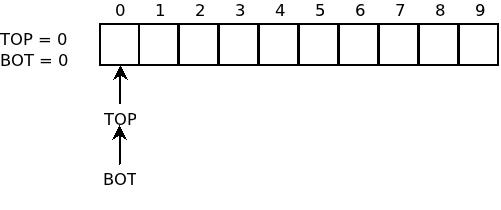
\includegraphics[width=\textwidth]{circ-init}
  \caption{
     \tiny The initial state of the circular array.
  }
  \label{fig:circ-1}
\end{subfigure}
~ %spacer
\begin{subfigure}[b]{0.31\textwidth}
  \centering
  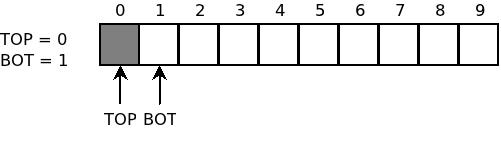
\includegraphics[width=\textwidth]{circ-push1}
  \vspace{1pt}
  \caption{
     \tiny The state after one de\_push\_bottom operation.
  }
  \label{fig:circ-2}
\end{subfigure}
~ %spacer
\begin{subfigure}[b]{0.31\textwidth}
  \centering
  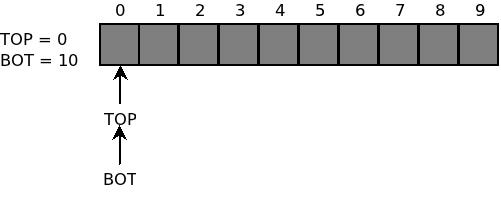
\includegraphics[width=\textwidth]{circ-push2}
  \caption{
    \tiny A further nine de\_push\_bottom operations. 
  }
  \label{fig:circ-3}
\end{subfigure}

\vspace{20pt}

\begin{subfigure}[b]{0.31\textwidth}
  \centering
  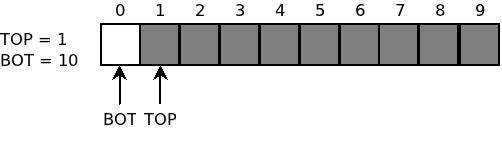
\includegraphics[width=\textwidth]{circ-steal1}
  \caption{
    \tiny 
  }
  \label{fig:circ-4}
\end{subfigure}
~ %spacer
\begin{subfigure}[b]{0.31\textwidth}
  \centering
  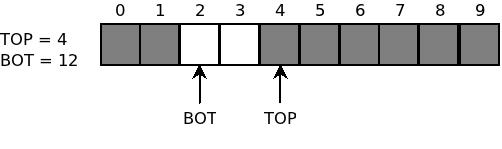
\includegraphics[width=\textwidth]{circ-stealpush1}
  \caption{
    \tiny 
  }
  \label{fig:circ-4}
\end{subfigure}
~ %spacer
\begin{subfigure}[b]{0.31\textwidth}
  \centering
  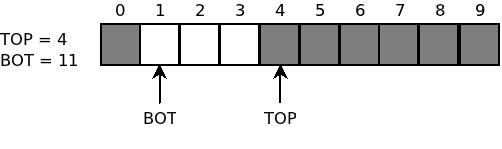
\includegraphics[width=\textwidth]{circ-pop1}
  \caption{
    \tiny 
  }
  \label{fig:circ-4}
\end{subfigure}

% full caption
\caption{
    A demonstration of the circular array data-structure. 
    The `TOP' field refers to the index of the top element of the deque and
    the `BOT' field refers to the index of the bottom element plus one.
    White squares indicate an un-used element, shaded squares indicate an
    element which is in use.
}
\label{fig:juliaimgs}
\end{figure}

\vspace{20pt}


% cicular array
The deque makes use of a \gls{circular array} which automatically grows and shrinks.
This approach is memory efficient and simple. 
It also allows for the top counter to remain unchanged unless a steal operation occurs (in most cases), reducing the frequency of locks occurring.
Figure \ref{fig:circ-demo} illustrates some of its mechanics. For instance figure \ref{fig:circ-5} shows that the array is circular, in that it
``wraps around" when the final element is reached and there are elements un-used at the start.

The design relies on bottom and top counters (used to index the array), the memory-size (the number of memory slots allocated to the deque), and 
the size (the number of elements which are currently used). The size is computed by subtracting the top counter from the bottom counter. 
This is used to detect an empty array, and detect when the array needs to be re-sized.
When the array is accessed the correct element is indexed by computing: \(realindex = index \bmod memorysize \). 
For example, let the top counter equal fifteen and the memory-size equal ten, the \(realindex\) of the top element is five.
This allows for the top and bottom counters to exceed the memory size and still point to the correct index, without allowing access to memory outside the 
bounds of the array. It also maintains that the size can be computed correctly. When the array becomes empty the counters are re-set to zero.

Should the size exceed the memory-size the array is automatically re-sized by double its current allocation. 
This is achieved by allocating a new array using malloc, copying the contents of the old array then freeing it, 
then assigning a pointer to the new array to the deque. 
Similarly, the array is shrunk by half when its size recedes to half of the memory-size using the same approach.
The consequence of this design is that the top\_mutex must be locked throughout the operation, blocking any de\_steal
attempts until the mutex is un-locked. 
The benefits of this approach are that the deque is more scalable and only memory that is likely to be used is allocated, 
rather than some amount that is defined at compile-time.

\subsubsection*{The Work-Stealing Mechanism}

% 4 key functions: 
% * ws\_worker\_thread
% * ws\_compute\_deque
% * ws\_become\_thief
% * ws\_victimise

\begin{itemize}
\item \textbf{ws\_worker\_thread: } \\
                The function which is passed to pthread\_create. This acts as the point of entry for each \gls{thread}.
                It accepts a pointer to the deque which is associated with the given thread\footnote{This is passed 
                in the form of a void pointer which has to be cast due to the interface provided by the pthreads
                library.}.
              
                This function makes use of a do-while loop which breaks when there is no work remaining in any \glspl{worker-thread} \gls{ready-deque}. 
                Each iteration of the loop sets the thread to work by calling the ws\_compute\_deque function, which returns when 
                no work remains in the \gls{ready-deque}. Then, the thread becomes a \gls{thief} and must attempt to acquire work
                from other threads by calling ws\_become\_thief. If more work is acquired the thread becomes a worker and calls ws\_compute\_deque
                again. If no work is found the condition for the loop are broken and the thread exits.
              
\item \textbf{ws\_compute\_deque: } \\
                Accepts a Deque pointer, i.e. to the Deque associated with the same thread. This function 
                calls de\_pop\_bottom until it detects that the ready-deque is empty, at which point it returns
                the total number of work items completed.
                
\item \textbf{ws\_become\_thief: } \\
                This operation randomly selects a thread to victimise. If it detects that there is no work
                available to steal it returns 0, otherwise it returns 1.
                It accepts a Deque pointer, i.e. to the Deque associated with the same thread. 
                
                When a victim is selected the ws\_victimise function is called.
                
                In order to determine that no work is available, a set to mark each thread which is unsuccessfully victimised (referred to as
                the exclude set) as-well as a counter is maintained.
                The exclude set is initialised adding the current thread. It is passed to the ws\_random\_deque
                \footnote{ws\_random\_deque uses 
                the standard c rand function to generate a number between zero and the number of threads to index an array 
                of deques and return one. An exclude set is passed to the function so that any member of that set is not returned.
                The function expects the exclude set to have at-least one element which is not asserted.}
                function. When the counter is equal to the number of threads one is returned.
                
\item \textbf{ws\_victimise: } \\
                
                
\end{itemize}

% ---------------------------------------------------------------------------------------------------------------------------------------------------------------
\subsection{A Render-Thread Work-Stealing Algorithm}

%to cover:
% * algorithm architecture: i.e. render threads, monitor thread.
% * Describe a steal operation.
% * Talk about initial distribution of work.
% * Talk about estimated completion time.

% ---------------------------------------------------------------------------------------------------------------------------------------------------------------
\section{Features for Demonstration}

%to cover:
% * Colour mandelbrot image which demonstrates work-stealing activity throughout execution.
% * Work-stealing trace mechanism.

% ---------------------------------------------------------------------------------------------------------------------------------------------------------------
\section{Validation and Verification}

% ---------------------------------------------------------------------------------------------------------------------------------------------------------------
% ---------------------------------------------------------------------------------------------------------------------------------------------------------------
% ---------------------------------------------------------------------------------------------------------------------------------------------------------------
\chapter{Discussion and Evaluation}
% ---------------------------------------------------------------------------------------------------------------------------------------------------------------
\section{Cross Analysis of the Implemented Algorithms}

% Show colour work-stealing images.
% Analyse trace output in graph form. i.e. Matrix size vs time for sequential, parallel, wsrandom, wsrenderthread.

% ---------------------------------------------------------------------------------------------------------------------------------------------------------------
\section{Reflection on Project}
\subsection{Further Work}

%to cover:
% * Cluster computation.
% * Adaption for use with more powerful architectures. 
% * More tracing abilities. 

% ---------------------------------------------------------------------------------------------------------------------------------------------------------------
% ---------------------------------------------------------------------------------------------------------------------------------------------------------------
% ---------------------------------------------------------------------------------------------------------------------------------------------------------------
\chapter{Resources}

\nocite{*}

% refs\bibs:
\bibliography{refs}

% ---------------------------------------------------------------------------------------------------------------------------------------------------------------
% ---------------------------------------------------------------------------------------------------------------------------------------------------------------
% ---------------------------------------------------------------------------------------------------------------------------------------------------------------

\chapter{Appendices}

\appendix
\chapter{Glossary of Terms}\label{sec:glosterm}

%\glsaddall
\printglossaries

\newpage
\chapter{Source Code}\label{sec:srccode}

\end{document}
